% !TEX root = ../../main.tex

\subsection{Nitrogen sorption at 77K}

Isotherms have been recorded on samples activated at both
\SI{200}{\degreeCelsius} and \SI{320}{\degreeCelsius}.
It is important to note that, as seen from the TGA curves,
not all capping agents leave the structure when thermal treating
at a lower temperature. The moieties which are still coordinated
to the Zr cluster will likely influence the adsorption
behaviour. At a high temperature, the dehydroxilation of the 
metal center also occurs~\cite{valenzanoDisclosingComplexStructure2011},
which may also affect the interaction with physisorbed probes. 
Several example isotherms can be found in
\autoref{def:fgr:n2phys-dataset}, with the complete dataset
present in \autoref{appx:def}, \autoref{appx:def:n2phys}.

There are a few isotherm features which can be analysed to
assess the type of modifications introduced in the structure
and their preponderence.

\begin{itemize}
	\item The slope of the isotherm at low \(p/p_0\) is representative
	      of the first interactions with the pore surface, which can be
	      quantified using the initial Henry constant. It will be influenced
		  by any changes in pore environment such as CUS or functionalised
		  defect sites.
	\item Missing liker defects will lead to an increase of the
	      apparent surface area and perhaps to a more extensive
	      pore network.
	\item The pore size distribution and total pore volume give
	      indications on the presence of missing cluster defects and/or
	      of the formation of mesoporous voids within the structure.
	\item A steep step at high \(p/p_0\) is indicative of intercrystal
	      condensation and suggests particle aggregation due to lower average
	      crystal size.
\end{itemize}

\begin{figure}[htbp]
	\centering

	\begin{subfigure}{0.45\linewidth}
		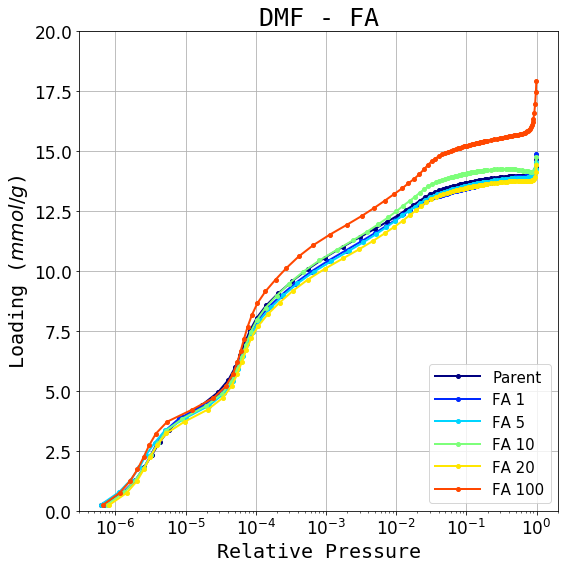
\includegraphics[width=\textwidth]{n2phys/dmf-fa}%
		\caption{}%
		\label{def:fgr:n2phys-dmf-fa}
	\end{subfigure}
	\begin{subfigure}{0.45\linewidth}
		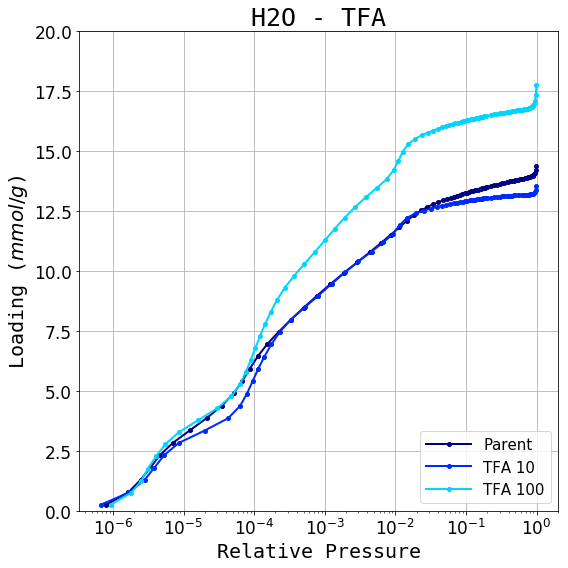
\includegraphics[width=\textwidth]{n2phys/h2o-tfa}%
		\caption{}%
		\label{def:fgr:n2phys-h2o-tfa}
	\end{subfigure}

	\begin{subfigure}{0.45\linewidth}
		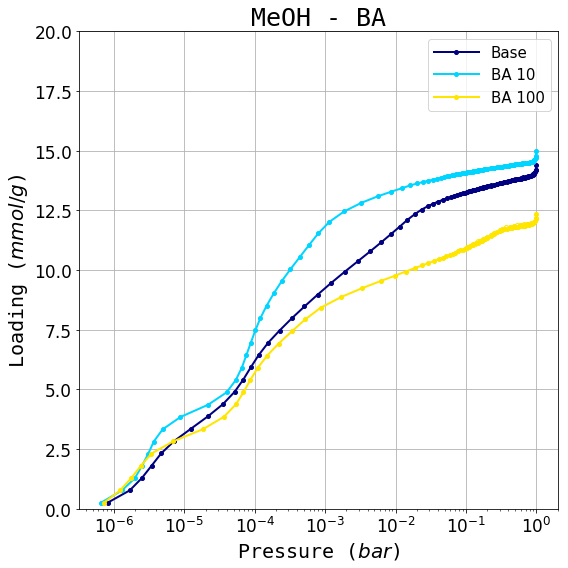
\includegraphics[width=\textwidth]{n2phys/meoh-ba}%
		\caption{}%
		\label{def:fgr:n2phys-meoh-ba}
	\end{subfigure}
	\begin{subfigure}{0.45\linewidth}
		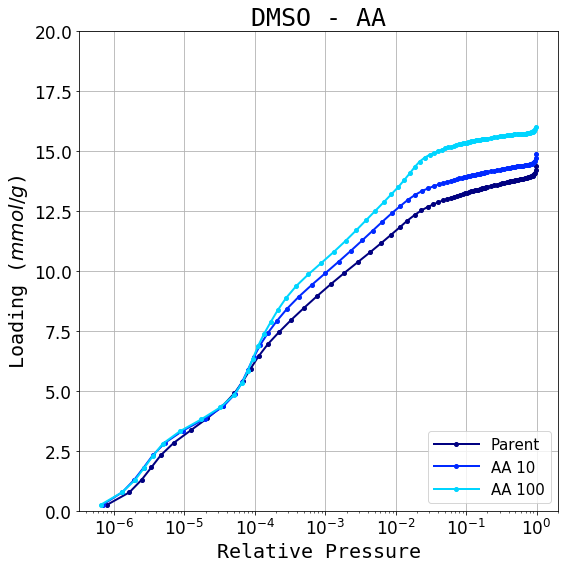
\includegraphics[width=\textwidth]{n2phys/dmso-aa}%
		\caption{}%
		\label{def:fgr:n2phys-dmso-aa}
	\end{subfigure}

	\caption{A selection of nitrogen sorption isotherms as measured on the
		leached samples at \SI{200}{\degreeCelsius}: (a) formic acid in DMF,
		(b) trifluoroacetic acid in water, (c) benzoic acid
		in methanol and (d) acetic acid
        in DMSO. The curve for the parent material is in dark blue.
        The x axis is logarithmic for clarity of low pressure 
        points.}%
	\label{def:fgr:n2phys-dataset}
\end{figure}

It is immediately apparent that the leaching process had an influence 
on the adsorption characteristics of UiO-66. Isotherms of acid treated
samples diverge from the parent material, often at different pressures.
In general, the total molar capacity at full loading is seen to increase,
a telltale sign of an increase in pore volume through defect generation.
On the other hand, other particularities exist, such as the benzoic acid
samples in methanol and DMSO where the low and high
concentration has opposite effect on the total loading. Predictors 
of defects and trends will be analysed in the following section.